%\documentclass{emulateapj}
%\documentclass[preprint2]{aastex}
% \documentclass[iop]{emulateapj}
\documentclass[useAMS,usenatbib]{mn2e}
\usepackage{epsfig}
\usepackage{epstopdf}
\usepackage{lscape} % Allows landscape environment to be used
\usepackage{graphicx}
\usepackage{multirow}
\usepackage{hhline}
\usepackage[fleqn]{amsmath}
\usepackage{gensymb}
\usepackage{commath}
%\usepackage{floatrow}
%\def\gtrsim{\mathrel{\hbox{\rlap{\hbox{\lower4pt\hbox{$\sim$}}}\hbox{$>$}}}}
%\renewcommand\floatpagefraction{.9}
%\renewcommand\dblfloatpagefraction{.9} % for two column documents
%\renewcommand\topfraction{.9}
%\renewcommand\dbltopfraction{.9} % for two column documents
%\renewcommand\bottomfraction{.9}
%\renewcommand\textfraction{.1}   
%\setcounter{totalnumber}{50}
%\setcounter{topnumber}{50}
%\setcounter{bottomnumber}{50}
\providecommand{\e}[1]{\ensuremath{\times 10^{#1}}}
\begin{document}

\title[Lensing Geometry]{
Pulsar Lensing Geometry
}

\author[Liu et al]{Siqi Liu$^{1,3}$\thanks{E-mail:\ sqliu@cita.utoronto.ca}, Ue-Li
  Pen$^{1,2}$\thanks{E-mail:\ pen@cita.utoronto.ca}, J-P Macquart$^{4}$\thanks{E-mail:J.Macquart@curtin.edu.au},
  Walter Brisken$^{5}$\thanks{Email:wbrisken@aoc.nrao.edu}, Adam Deller$^{6}$\thanks{E-mail:deller@astron.nl}\\
 $^1$ Canadian Institute for Theoretical Astrophysics, University of Toronto, M5S 3H8 Ontario, Canada \\
$^2$ Canadian Institute for Advanced Research, Program in Cosmology
and Gravitation\\
$^3$ Department of Astronomy and Astrophysics, University of Toronto, M5S 3H4, Ontario, Canada\\
$^4$ ICRAR-Curtin University of Technology, Department of Imaging and Applied Physics, GPO Box U1978, Perth, Western Australia 6102, USA \\
$^5$ National Radio Astronomy Observatory, P.O. Box O, Socorro, NM 87801, USA\\
$^6$ ASTRON, the Netherlands Institute for Radio Astronomy, Postbus 2, 7990 AA, Dwingeloo, The Netherlands\\
}

\date{\today}

\pagerange{\pageref{firstpage}--\pageref{lastpage}} 
\pubyear{2015}

\maketitle
\label{firstpage}
\begin{abstract}
We analyze archival VLBI data of PSR
B0834+06, concluding that for this example the plasma lenses can be
precisely modelled using the inclined sheet model \citep{2014MNRAS.442.3338P},
resulting in two distinct lens planes.  This data strongly favours the
grazing sheet model over turbulence as the primary source of
pulsar scattering.  7 observed apex parameters fit the model to percent accuracy.
The simple 1-D structure of the lenses opens up
the possibility of using interstellar lenses as precision probes for
pulsar lens mapping, and new opportunities for removing scattering to
improve pulsar timing.
We describe the parameters and observables of this double screen
system.  While relative screen distances can in principle be
accurately determined,
a global conformal distance degeneracy exists which allows a rescaling
of the absolute distance scale.  This degeneracy is broken if the
pulsar resides in a binary system, which is the case for most
precision timing targets.

\end{abstract}
\begin{keywords}
Pulsar
\end{keywords}

\newcommand{\be}{\begin{eqnarray}}
\newcommand{\ee}{\end{eqnarray}}
\newcommand{\beq}{\begin{equation}}
\newcommand{\eeq}{\end{equation}}

\section{Introduction}

Pulsars have long provided a rich source of astrophysical information
due to their compact emission and predictable timing. One of the
weakest measurements for most pulsars is their direct geometric
distance.  For some pulsars, timing parallax or VLBI parallax has
resulted in direct distance determination.  For most pulsars, the
distance is a major uncertainty for precision timing interpretations,
including mass, moment of inertia\citep{2006Sci...314...97K,2012hpa..book.....L}, and
gravitational wave direction \citep{boyle2012}.

Direct VLBI observation of PSR B0834+06 shows multiple images lensed
by the interstellar plasma.  Combining the angular positions and
scintillation delays, the authors published the derived effective
distance \citep{2010ApJ...708..232B} of approximately $1168\pm 23$ pc
for apexes on the main scattering axis.
%, and $1121\pm 59$ pc for $1$ ms apexes.  
This represents a precise
measurement compared to all other attempts to derive distances to this
pulsar.  This effective distance is a combination of pulsar-screen and
earth-screen distances, and does not allow a separate determination of
the individual distances.  A binary pulsar system would in principle
allow a breaking of this degeneracy \citep{2014MNRAS.442.3338P}. One
potential limitation is the precision to which the lensing model can
be understood.  In this paper, we demonstrate that the lensing screen
consists of nearly parallel linear refractive structures, in two
screens.  The precise model confirms the one dimensional nature, and
thus the small number of parameters that
quantify the lensing screen. 

\section{Lensing}

In this section we map the data onto the grazing incidence sheet
model.  The folded sheet model is qualitatively analogous to a
reflection of a street lamp on a lake as seen from the other shore.  In the
absence of waves, exactly one image forms at the point where the angle
of incidence is equal to the angle of reflection.  In the presence of
waves, one generically sees a line of images above and below the
unperturbed image.  A similar effect occurs when the observer is below
the surface.  Two major distinctions arise: 1. the waves can deform
the surface to create caustics in projection. Near caustics, Snell's
law can lead to highly amplified refraction angles. 2. due to the odd
image theorem, each caustic leads to two images.  In practice, the
surface could be caused be reconnection
sheets\citep{2015MNRAS.450.3201B}, which have finite widths to
regularize these singularities. Diffusive structures have Gaussian
profiles, which was analyzed in \citet{2012MNRAS.421L.132P}.

The generic interstellar electron density is insufficient to deflect
radio waves by the observed $\sim$ mas bending angles. At grazing
incidence, Snell's law results in an enhanced bending angle, which
formally diverges.  Magnetic discontinuities generically propagate
as transverse surface waves, whose restoring force is the change in Alven
speed on the two sides of the discontinuity. This completes the
analogy to waves on a lake: for sufficiently inclined sheets the waves
will appear to fold back onto themselves in projection on the sky.  At
each fold caustic, Snell's law diverges, leading to enhanced
refractive lensing.  The divergence is cut off by a finite width of
the sheet.  The generic consequence is a series of collinear images.
Each fold of the wave results in two density caustics.  Each density
caustic leads to two geometric lensing images, for a total of 4 images
for each wave inflection.  The two geometric image in each caustic are
separated by the characteristic width of the sheet, if this is smaller
than the Fresnel scale, the two images become effectively
indistinguishable. 

A large number of sheets might intersect the line of sight to any
pulsar. Only those sufficiently inclined would lead to caustic
formation. Emprically, some pulsar scattering appears dominated by a
single sheet, leading to the prominent inverted
arclets\citep{2001ApJ...549L..97S}.

\subsection{Archival data of B0834+06}
\label{21}
%Our analysis is based on the reduced apex catalog from
Our analysis is based on the apex data selected from the secondary
spectrum of pulsar B0834+06 in \citep{2010ApJ...708..232B}, which was
observed as part of a 300 MHz global VLBI project on 2005 November 12, with
GBT (GB), Arecibo (AR), Lovell and Westerbork (WB) telescopes.  The GB-AR and AR-WB
baselines are close to orthogonal and of comparable lengths, resulting
in relatively isotropic astrometric positions.
Information from each identified apex includes delay $\tau$,
delay rate (differential frequency $f_D$), relative Right Ascension
$\Delta\alpha$ and relative declination $\Delta\delta$.
%$, error of $\Delta\alpha$ $\sigma_{\alpha}$ and error of
%$\Delta\delta$ $\sigma_{\delta}$. 
Data of each apex are collected from four dual circular polarization $8$ MHz wide sub-bands spanning the frequency range $310.5$--$342.5$ MHz. 
As described in \citet{2010ApJ...708..232B}, the inverse parabolic
arclets were fitted to positions of their apexes, resulting in a
catalog of apexes in each sub-band, each with delay and differential
frequency.  As previously described, the positions of the apexes
apears constant across sub-bands.  In this work, we first combine the
apexes across sub-bands, resulting in a single set of images.  We focus on
the southern group with negative differential frequency: this
grouping appears as a likely candidate for a double lensing screen
since two groups appear distinct in both the VLBI angular positions, and the
secondary spectra.
We divide the apex data with negative differential frequency into two
groups: in one group time delay ranges from $0.1$ ms to $0.4$ ms,
which we call $0.4$ ms group, and in the other group time, delay at
about $1$ ms, which we call $1$ ms group.  In summary, the
$0.4$ ms group contains $10$ apexes in the first two sub-bands, and $14$ apexes in the last two sub-bands; the $1$ ms group, contains $5$, $6$, $5$ and $4$ apexes in the four sub-bands subsequently, with center frequency $f_{\rm band}=314.5, 322.5, 330.5$ and $ 338.5$ MHz. 

We select the equivalent apexes from four sub-bands. To match the same apexes in different sub-bands, we scale the differential frequency in different sub-bands to $322.5$ MHz, by $f_D/f_{\rm band}\cdot322.5$ MHz. We map
a total of $9$ apexes from the $0.4$ ms group, and $5$ apexes from the $1$ ms
group. This results in an estimation
for the mean referenced to $f=322.5$ MHz and a standard deviation among four sub-bands. They are listed in Table
\ref{table:apex}. The $f_D$ and $\tau$ are the  mean of the four sub-bands. 
%$\bar{x}={\sum\limits^{n=4}_{i=1}{x_i}}/{4}$, x is for $f_D$ or $\tau$.
The mean value of $\Delta\alpha$ and $\Delta\delta$ are the weighted mean.
% calculated by following equation:
%\begin{align*}
%x=\sum\limits^{n=4}_{i=1}\frac{x_i}{{\sigma_i}^2},
%\end{align*}
%Here x is for $\Delta\alpha$ or $\Delta\delta$. 


\begin{table*}
\centering
%\label{apex1ms}
%\resizebox{1cm}{!}{
\begin{tabular}{llllll}
\hline
$\theta_{1\parallel}$(mas) & $f_D$(mHz) & $\tau$(ms)  & $\Delta\alpha$(mas) & $\Delta\delta$(mas) & $t_0$(days)\\
\hline
 -8.26   & -12.9(2)      & 0.0845(5) & 2.9(3)  & -8.2(4)      & -48.7                                \\
-10.68   &-16.8(3)      & 0.1412(9)  & 3.9(6) & -10.6(4)      &-62.8                                \\
-12.32   &-18.9(2)      & 0.188(2)   & 5.1(6) & -10.6(6)      &-74.2                        \\
-13.41 & -20.4(5)      & 0.222(3)     & 5.6(3)  & -11.73(8)    &-81.4                                \\
-13.82 &-21.2(6)        & 0.236(2)    & 5.1(4)  & -12.6(5)      &-83.3                                \\
-14.59   &-22.3(5)      & 0.2633(3)    & 6.2(3)  & -14.2(7)     &-88.1                                \\
-16.24   &-24.6(4)       & 0.327(3)   & 6.5(6)  & -14.1(4)       &-99.0                                \\
-16.52  &-24.9(4)      & 0.3378(3)         & 8.3(4)  & -14.4(8)      &-101                                \\
-17.39   &-26.1(4)    & 0.3743(6)         & 8.5(3)    & -15.7(3)      &-107                               
\\ \hline
$\cdots$&         -35.1(5)  & 0.950(2)   & -15(1)  & -21(1)   &-202                                   \\
$\cdots$ & -38.3(6)  & 0.9763(9)   & -15(1)       & -20.7(3)  &-190                                    \\
$\cdots$ & -40.2(6)  & 1.005(8)    & -14(1)       & -22.3(4)  &-187                                   \\
$\cdots$ & -41.3(5)    & 1.037(3)   & -11(1)     & -19(3)   &-188                                   \\
$ \cdots$ & -43.1(4)      & 1.066(5)    & -8(3)     & -24(2)   &-185   \\
 \hline                                 
\end{tabular}
%}
\caption{ $0.4$ ms and $1$ ms reduced apex data. 
The upper part of the table list the $0.4$ ms group data, while the $1$ ms group lie in the lower part of the table. 
Observation data include the differential frequency $f_D$, time delay
$\tau$ ($\tau_1$ for $0.4$ ms group and $\tau_2$ for $1$ ms group);
$\Delta\alpha$ and $\Delta\delta$ are from the VLBI measurement. 
$t_0$ is the time at constant velocity for an apex to intersect the
origin at constant speed along the main scattering parabola.  More
details in Section \ref{21}.
%The methods of how to calculate the error of time delay, differential
%frequency and the last column time are mentioned in Section \ref{21}.
}
% $\theta_{1\parallel}$, the angle of the $0.4$ ms group with the component in the axis defined by $\gamma$, are derived from the $\theta-\tau$ relation plotted in Figure \ref{thetata}
\label{table:apex}
\end{table*}



The method we use to calculate the error of time delay $\tau$, differential frequency $f_D$, $\Delta\alpha$ and $\Delta\delta$ are listed in Table \ref{table:apex}, is by following equation:
\begin{equation}
\begin{aligned}
\sigma^2_{\rm \tau, f_D,\Delta\alpha, \Delta\delta} = \frac{\sum\limits^{4}_{i=1}(x_i-\bar{x})^2}{n(n-1)},
\end{aligned}
\end{equation}
and $n=4$ for four sub-bands.
% This is also how we calculate the sample error of $\Delta\alpha$ and $\Delta\delta$, marked with errorbars in Figure \ref{Doublelens}.

%For the circles in Figure \ref{Doublelens}, they are calculated by following equation:
%\begin{equation}
%\begin{aligned}
%(\frac{1}{\sigma_{\rm \alpha, \delta}})^2 = \sum\limits^{n=4}_{i=1}{\frac{1}{{ \rm \sigma_i}^2}}.
%\end{aligned}
%\end{equation}
%where $\rm \sigma_i$ is the error of the data in each sub-band. They are marked with circles in Figure \ref{Doublelens}.

\subsection{One lens model}
\subsubsection{Distance to the lens}
In the absence of a lens model, the
fringe rate, delay and angular position cannot be uniquely related. To interpret the data, we adopt the lensing model of
\citep{2014MNRAS.442.3338P}.  In this model, the lensing is due to projected fold caustics of a thin sheet closely aligned to the line of sight. 

%How the distance of the pulsar $D_p$ and the time delay $\tau$ and angular offset $\theta$ are matched, and how velocity and the differential frequency $f_D$ are matched, are related by the following equations:


%The relation of the distance of the pulsar $D_p$, the time delay
%$\tau$ with the angular offset $\theta$, and the relation of velocity
%and the differential frequency $f_D$ are described by the following
%equations:

We define the {\it effective distance} $D_{\rm e}$ as
\begin{equation}
D_{\rm e} \equiv \frac{2c\tau}{\theta^2}.
%f_D  &=f\frac{\rm d\tau}{\dif t},
\end{equation}
The differential frequency is related to the rate of change of delay
as $f_D  =-f\frac{\rm d\tau}{\dif t}$.  The effective distance
corresponds to the pulsar distance $D_{\rm p}$ if the screen is exactly halfway.
In general, $D_{\rm e}={D_{\rm p} D_{\rm s}}/({D_{\rm p} - D_{\rm
    s}})$ for a screen at $D_{\rm s}$.


%analysis of the effective distance follows:
%\begin{equation}
%\begin{aligned}
%k{\sum\limits_{i=1}^n\frac{1}{\sigma_{ki}^2}}&=\sum\limits_{i=1}^n\frac{\theta/\sqrt%{\tau}}{\sigma_{ki}^2},\\
%\frac{1}{\sigma_k^2}&=\sum\limits_{i=1}^n\frac{1}{\sigma_{ki}^2},
%\end{aligned}
%\end{equation}
%where $k$ is denoted as the slope in Figure \ref{thetatau}, and
%$\sigma_{ki}$ as the error of the slope. $\sigma_{ki}=\sigma_{\theta
%  i}/\sqrt{\tau}$,
%$\sigma_{\theta}=\sqrt{(\sigma_{\Delta\alpha}{\cos(\delta)})^2+\sigma_{\Delta\delta}%^2}$. $n=9$
%for $1$ ms group, and $n=4$ for $0.4$ ms group. 

\begin{figure}
\centering
%\epsscale{1.0}
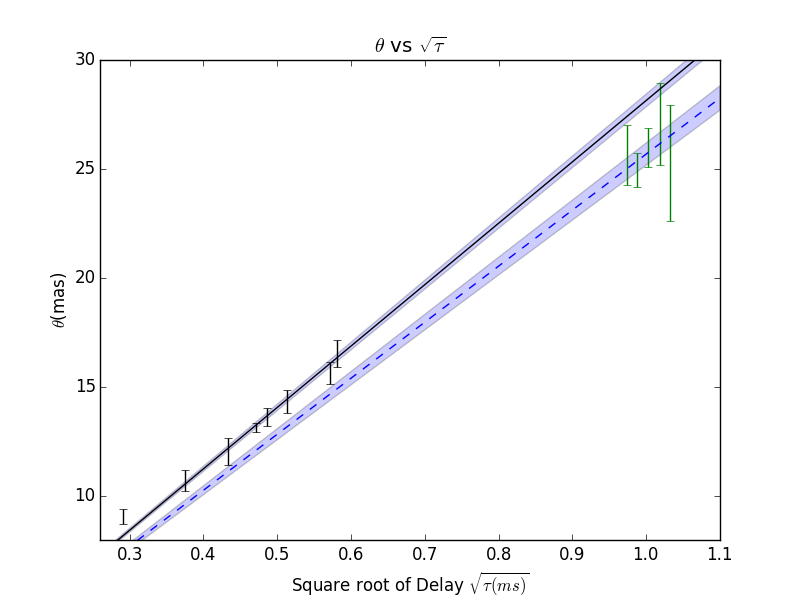
\includegraphics[width=1.0\linewidth, angle=0]{Theta_tau.png}
\caption{${\theta}$ vs ${\sqrt{\tau}}$. Two separate lines through the
  origin were fitted to the points sampled among the $0.4$ ms group
  and $1$ ms group. The solid line is the fitted line of the $0.4$ ms
  positions, where $D_{1\rm e}=1013$ pc with an error region of
  $\sigma_D=27$ pc. The dashed lines are the fitted lines of the $1$ ms
  position, where $D_{2\rm e}=1281$ pc with an error region
  $\sigma_D=82$ pc.
}
\label{thetatau}
\end{figure}


In the angular offset of the scintillation image away from the central
emission we subtract the expected noise bias:
${\theta}^2=({\Delta\alpha}\cos(\delta))^2+({\Delta\delta})^2-\sigma^2_{\Delta\alpha}-\sigma^2_{\Delta\delta}$. 
We plot the $\theta$ vs square root of $\tau$ in Figure
\ref{thetatau}. A least square fit to the distance results in
$D_{1{\rm e}}=1023\pm 27$ pc for the  $0.4$\ ms group, which we call lens 1, and
$D_{2{\rm e}} = 1281 \pm 82$ pc for the $1$\ ms group, hereafter lens 2.
The errors, and uncertainties on the error, precludes a definitive
interpretation of the apparent difference in distance.  At face value, 
this indicates that the lens 2 is closer to the pulsar, and we will
use this as a basis for the model in this paper.  We discuss
consequences of alternate interpretations in section \ref{sec:degeneracy}.
%The error bars are large enough to allow them to be at the same
%distance, or perhaps a reverse distance ordering.  In this paper, we
%present two analyses for comparison: equidistant, and at the best fit
%distances. In the first case, no direct distance measurement is
%possible, but it nevertheless illustrates a robust interpretation of
%the data.
The pulsar distance was directly measured using VLBI parallax to be
$D_{\rm p} = 625 \pm 59$ pc.  For modelling purposes, we will use
$D_{\rm p} = 640$ pc, consistent with the direct measurement.  Similarly,
we take $D_{1{\rm e}}=1023$ pc,  and the distance of lens 1 $D_{1}$,
where $0.4$ ms scintillation points are refracted, is equal to $393.7$
pc. For $1$ ms apexes, the distance of lens 2 is taken as $426.7$ pc,
slighly closer to the pulsar.
%From time delay $\tau$ and the angular position of the pulsar, we obtained the effective distance of the pulsar as follows: 
%for $0.4$ ms group, $D_{\rm e}=1017\pm2.8$\ pc; 
%and for $1$ ms group, $D_{\rm e}=1121\pm64$\ pc.

%\subsubsection{Angular positions of $0.4$ ms group}
%\label{subsec:angularpos}

For the 0.4 ms group, we adopt the geometry from
\citet{2010ApJ...708..232B}, assigning these points along line AB as
shown in Figure \ref{Doublelens} based solely on their delay, which is
the best measured observable. The line AB is taken as a
fixed angle of $\gamma=-25.2\degree$ east of the
declination axis. We use this axis
to define ${\parallel}$ and define ${\bot}$ by a $90\degree$ clockwise
rotation.  


\begin{figure*}
\centering
%\epsscale{1.0}
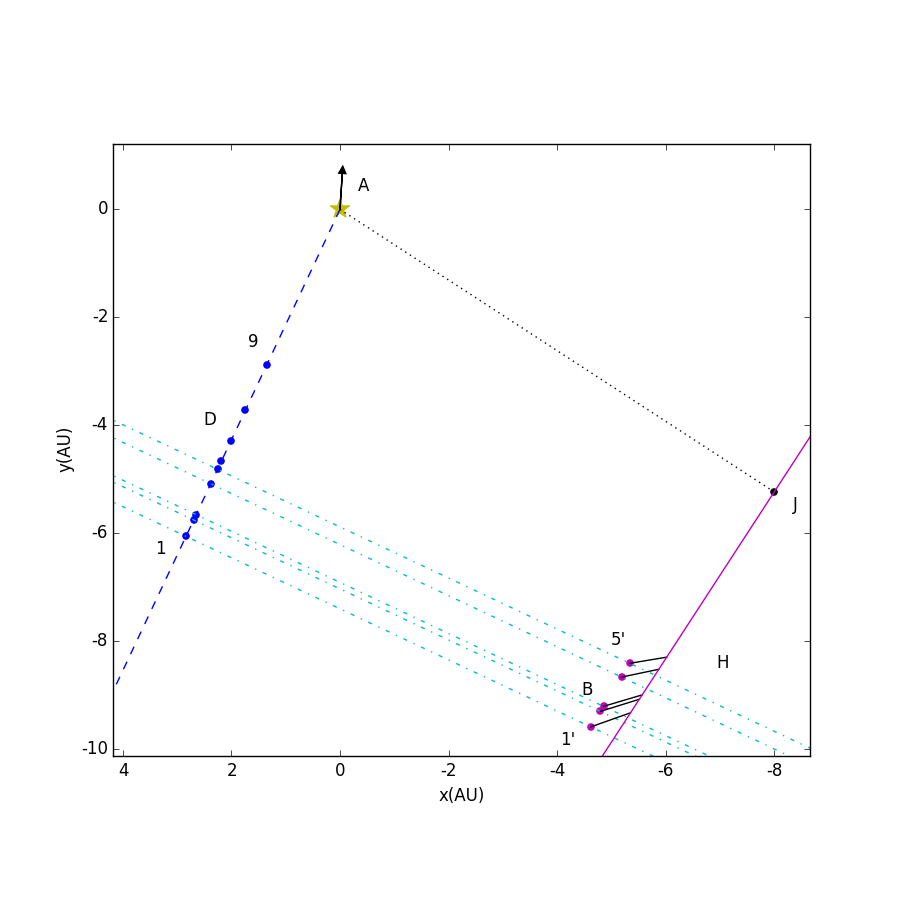
\includegraphics[width=1.0\textwidth, angle=0]{Double_lens_xy.png}
\caption{Model angular positions of $0.4$ ms and $1$ ms data in the double
  lens model. x axis and y axis are the relative distance to central
  emission of pulsar in Right Ascension direction and declination
  direction, on a 2D plane that is transverse to the line of
  sight. The screen distances are $393.7$ pc and $426.7$ pc for left and
  right groups
  respectively. Scatter points on the left side, marked with letter
  D, are the calculated positions from the $0.4$ ms apexes
  observation. The dashed line aligns the $0.4$ ms apexes
  positions, with a angle $\gamma=-25.2\degree$  east of north. The
  scatter points on the right side, marked with letter B, are the
  calculated lensed image on lens 1 from $1$ ms group. The short solid
  line connects the lensed image one lens 1(observable) and lensed
  image 2(unobservable), marked with letter H. Long solid line is the
  fitted line of these positions. The dotted line on the top right
  side is perpendicular to the solid line, intersecting at J. Short
  light solid lines connect the model apparent image positions to the
  position of the first scattering for the $1$ ms group. Dot dash
  lines are perpendicular to the 
  AD scattering axis.  They connect the $0.4$
  ms and $1$ ms calculated positions with the same
  $\theta_{1\parallel}$, which are denoted as lens 1. The proper
  motion of the pulsar is $192.4$ km/s, with an angle
  $\epsilon=-4.34\degree$ east of north, is marked with an arrow from
  the star, point A the position of the pulsar, at the top of the
  figure.} 
\label{Doublelens}
\end{figure*}



%We calculate $\theta$ from the $\theta$--$\sqrt{\tau}$ relation and observed $\tau$. Because all of the $\theta$ here lie on the axis defin%ed by $\gamma$ on lens 1, so they are also denoted $\theta_{1\parallel}$ listed in the first column in Table \ref{table:apex}. Then the calc%ulated angular positions of the $0.4$ ms group are calculated:
%\begin{equation}
%\begin{aligned}
%{\Delta\alpha_C}&=-\theta {\sin}\gamma/\cos{\delta}, \\
%{\Delta\delta_C}&=-\theta {\cos}\gamma,
%\end{aligned}
%\end{equation}
%which are marked out with the scatter points on the left side in Figure \ref{Doublelens}.


%\subsubsection{Angular positions of $1$ ms group}
%To calculate the angular positions of the $1$ ms group, we do it in following steps. 

%First, with observed $\tau$ and matching the $\theta-\sqrt{\tau}$ relation, which is plotted in Figure \ref{thetatau}, the angular offset $\theta$ is obtained. 
%Note that we define the velocity that is in the direction of the pulsar. 

%Second, we consider the point with the largest $\theta$ among this $1$ ms group, denoted as 5, shareing the same $\theta_{\parallel}$ with the point with the largest $\theta$ among the $0.4$ ms group, represented as 6. $\theta_{\bot}$ is calculated by $\theta_{\bot}=\sqrt{\theta^2-\theta_{\parallel} ^2} $. Then, by using a rotation matrix defined by $\gamma$, the position of point 5 is determined: $(-10.36,-24.10)$ mas. 

%Third, to determine the position of the rest points $1-4$, we need to know the velocity of the pulsar, and then fit the calculated $\Delta\alpha_C$ and $\Delta\delta_C$ to get the same differential frequency with the observation. To know the velocity of the pulsar, we calculated the velocity component in two directions: ${v_\parallel}$ according to the differential frequency of point $6$ in $0.4$ ms group and ${v_\bot}$.

%, the parallel direction is defined by the the axis that is $\gamma$ away from declination axis. 
%$v_{\rm A5}$ (in the direction pointing from point 5 to A), which has the component in the transverse direction of the velocity can be used to calculate $v_{\bot}$, with the differential frequency $f_D$ of point $5$. The example of how the lensed image changes with the moving of the pulsar is plotted in Figure \ref{OneLensReflect}. More specifically, in a time period of $6500$ s ($\rm dt=6500$ s), we will solve two equations:
%\begin{equation} 
%\begin{aligned}
%{\rm d\tau}&=\tau(t=0{\rm s})-\tau(t=6500~{\rm s},v_{\parallel})&=f_{\rm D6}/f\cdot{\rm dt},\\
%{\rm d\tau}&=\tau(t=0 {\rm s}) -\tau(t=6500~{\rm s}, v_{\rm A5}) & = f_{\rm D5} /f\cdot{\rm dt},
%\end{aligned}
%\end{equation}
%where $f=322.5$ MHz. With the calculated $v_{\rm A5}$, we can calculate the $v_{\bot}$. Combining the $v_{\parallel}$, the total velocity of the pulsar $v_{\rm tot}$ and its angle with the north (declination) axis $\epsilon$. The result is $v_{\parallel}=179.8$ km/s and $v_{\rm A5}=161.8$ km/s. Thus the total velocity is $188.6$ km/s and $\epsilon=-7.45\degree$.

%Fourth, we fit the positions of the rest four points, with known proper motion of the pulsar. For example, point 4:
%\begin{equation}
%\begin{aligned}
%\frac{f_{\rm D4}}{f}&=\frac{\tau(t=0 {\rm s})-\tau(t=6500~{\rm s}, v_{\rm A4})}{\rm dt} ,\\
%\frac{v_{\rm A4}}{v_{\rm tot} }&=\frac{\Delta\alpha\cdot\sin{\gamma}}{\sqrt{(\Delta\alpha)^2\cos^2(\delta)+(\Delta\delta)^2}}+\frac{\Delta\delta\cdot\cos{\gamma}}{\sqrt{((\Delta\alpha)^2\cdot\cos^2(\delta)+(\Delta\delta)^2}}
%\cdot[ { \sin( {\tan}^{-1}(\alpha,\delta))\cos(\gamma)}-\cos({\tan}^{-1}(\alpha,\delta))\sin(\gamma)]. \\
%{\alpha}^2+{\delta}^2 &= {\theta}^2
%\end{aligned}
%\end{equation}
%We fit a line to this five calculated points to describe the the positions of these 5 points. 
%Lying on the fitted line, point 5 share the same $\theta_{\parallel}$ as the point with the largest $\theta_{\parallel}$ in the $0.4$ ms apexes. Solving the differential frequency ${f_D}$ of this point, we can calculate the relative velocity of this point to the pulsar, called vA2, which is in the plane that is perpendicular to our line of sight with a direction pointing from point 5 to the position of the pulsar. With the same method, we obtained the $v_{\parallel}$ from the $0.4$ ms data. Thus, the total velocity of the pulsar is determined.

%While this one lens does not fit the data, we will abandon the velocity calculated in this model.

%\begin{figure}
%\centering
%\epsscale{1.0}
%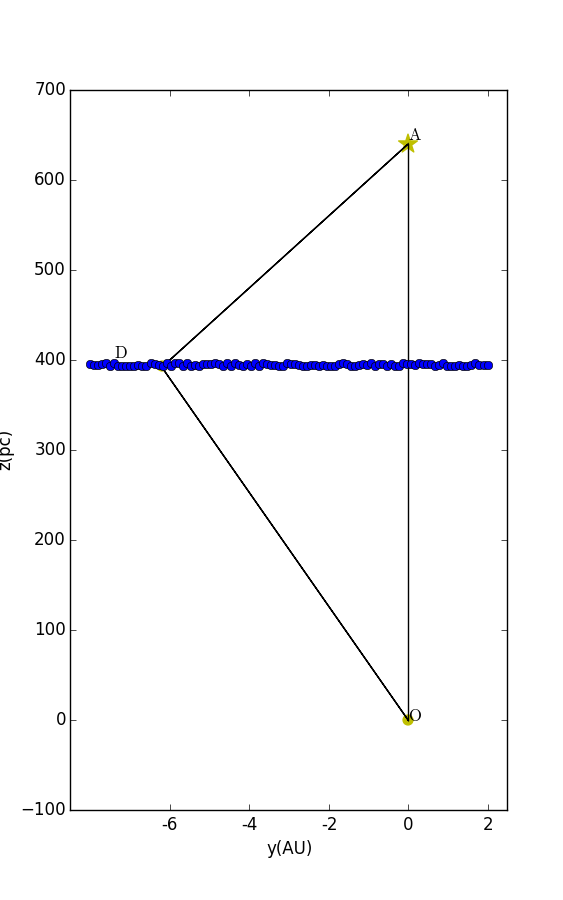
\includegraphics[width=1.0\linewidth, angle=0]{One_lens_light_path.png}
%\caption{This shows the light path of lensed/ unlensed image. The solid line on the right is the light directly emits from the pulsar to the observer. The two solid lines on the left are the lensed path. The curved line in the middle is the where lens 1 lie. X axis represents the distance in declination direction, and y axis represents the radial distance.}
%\label{OneLensLightPath}
%\end{figure}


\subsubsection{Discussion of one lens model}

The $0.4$ ms group lens solution appears consistent with the premise
of the inclined sheet lensing model \citep{2014MNRAS.442.3338P}, which
predicts collinear positions of lensing images.  The time in last
column of Table \ref{table:apex}, which we denote as $t_0$, is
calculated with $-2{\tau}f/{f_{D}}$, corresponds to the time required
for the delay of an arclet to cross zero.

The collinearity can be considered a postdiction of this model.  The
precise positions of each image is random, and with 9 images no
precision test is possible.  The predictive power of sheet model
becomes clear in the presence of a second, off-axis, screen.  This
will be discussed below.

%Knowing time delay ${\tau}$, we can calculate the distance of the screen; knowing the angular position of point 5 and its differential frequency ${f_D}$, we can get the velocity of the pulsar; knowing the velocity and observation differential frequency, we can get the position of points $1$--$4$. 

%\begin{figure}
%\centering
%%\epsscale{1.0}
%\includegraphics[width=1.0\linewidth, angle=0]{One_lens_reflection.png}
%\caption{The moving of the lensed image with the moving of the pulsar. x axis and y axis are the relative distance to the central emission of the pulsar. $A_1$ is the original position of the pulsar, and $A_2$ is the position of the pulsar after 650000s (7.5 days). Dashed line describes the incoming light. Dotted line is the place where lensed image on lens 1 lies. $D_2$ is the place where the lensed image lie when the pulsar moved to $A_2$.}
%\label{OneLensReflect}
%\end{figure}

\subsection{Double lens model}
\label{doublelensmodel}

The apparent offset of the 1ms group can be explained by a second lens
screen.  The small number of apexes at 1ms suggests that the second
lens screen involves a single caustic at a different distance.  In the
primary lens system, the inclination appears such that typical waves
form caustics.  The number of sheets at more shallow inclination
increases as the square of the small angle.  A 3 times less inclined
sheet occurs 9 times as often.  If a 1-$\sigma$ wave forms a caustic
in the primary lens, a 3 times less inclined surface only forms
caustics for 3-$\sigma$ waves, which occur two hundred times less
often.  Thus, one expects such sheets to only form isolated caustics,
which we expect to see occasionally.  Three free parameters describe a
second caustic: distance, angle, and angular separation.  We fix the
distance from the effective VLBI distance, and fit the angular
separation and angle using the 5 delays of the 1ms group.

\subsubsection{Solving the double lens model}
%The $v_{\parallel}$ to the plane should be equal. While for the calculated positions of $1$ ms apexes, they do not. 
We denote the position of the pulsar point A, position of the lensed image on lens 2 point H, position of the lensed image on lens 1 point B, position of the observer point O, perpendicular from the pulsar to line HJ point J, the perpendicular from point H to line BD point F, and the perpendicular from point B to line HJ point G, for easier discussion.
%As what Figure \ref{first_reflect} shows, AH should be perpendicular to HE, lens 2. 
%The plane where the light was refracted should be transverse to the line that connects the pulsar and the lensed image. 
Because points $1-4$ share the approximately same time delay with point $5$, the lens where the image formed should be at the same distance away from us. The only reasonable position of screen (line HJ) that fits all these five points, marked with a solid line in Figure \ref{Doublelens}.  
%However, in this senario, the screens cross each other, which means HE crosses with each other. 
%That is unrealistic for the structure of the interstellar medium. 
%Thus, on the plane which is perpendicular to our line of sight, the incoming line should be in agree with the refraction line.
% If the light of the pulsar are being refracted by one interstellar medium lens, they should be distributed along a line like the axis of the $0.4$\ ms group, and we already know that all $1$ ms lensed images lie on the solid line in Figure \ref{Doublelens}, the only possible position will be J, which is the perpendicular of the position of the pulsar to the screen. 

%Therefore, we consider another model candidate: the double lens model. Respective cal%culation shows that the light is first refracted by lens 2 and then refracted by lens 1. 

The first step is to calculate the position of J. We make an estimate of the distance of J by the $1$ ms $\theta$--$\sqrt{\tau}$ relation, and then we calculated the position of J by matching the time delay of point 2 and point 5. The result shows that lens 2 is $426.7$ pc away from us. And its position is marked in Figure \ref{Doublelens}. Because J is the perpendicular to lens 2, we made a line that is perpendicular to AJ, the solid line in Figure \ref{Doublelens} to denote lens 2.
%calculate the position of the far lens (lens $1$) and the near lens (lens $2$). As what has been discussed previously, the solid line is considered to be the far lens, where the positions have a larger effective distance. And the near lens is considered to be the lines that is perpendicular to the $0.4$ ms group axis. 

The second step is to find the matched pairs of those two lenses. By
inspection we found that the 5 furthest points in $0.4$ ms group match
naturally to the double lens images.  These five matched lines are marked with dot dash lines in Figure \ref{Doublelens} and their values are listed in the first two columns in Table \ref{table:double_lens_compare}. They are the located at a distance $393.7$ pc away from us. Here we define three distances:
\begin{equation}
\begin{aligned}
D_{p2}&=640~{\rm pc}-426.7~{\rm pc} =213.3~{\rm pc},\\
D_{21}&=426.7~{\rm pc}-393.7~{\rm pc} =33.0~{\rm pc},\\
D_{1}&=393.7~{\rm pc}- 0~{\rm pc} = 393.7~{\rm pc}, 
\end{aligned} 
\end{equation}
where $D_{p2}$ is the distance from the pulsar to lens 2, $D_{21}$ is the distance from lens 2 to lens 1, and $D_{1}$ is the distance from lens 1 to the observer.
%We calculated with the distance of the screen which is calculated in the one lens model, and then move the distance of the far screen little by little to make the calculated time delay match the observation resul

Figure \ref{first_reflect} and Figure \ref{second_reflect} are examples of how light are being refracted on the first lens plane and the second lens plane. We specifically chose the point with $\theta_{1\parallel}$ equal to $-17.39$ mas, which is point 5 on lens 2 and point 6 on lens 1 as an example. We solve the solutions in double lens model by following equations:
\begin{equation}
\begin{aligned}
\frac{\rm JH}{D_{p2}}&=\frac{\rm HG}{D_{21}},\\
\frac{\rm FB}{D_{21}}&=\frac{\rm BD}{D_{1}}.
\end{aligned}
\end{equation}


\begin{figure}
\centering
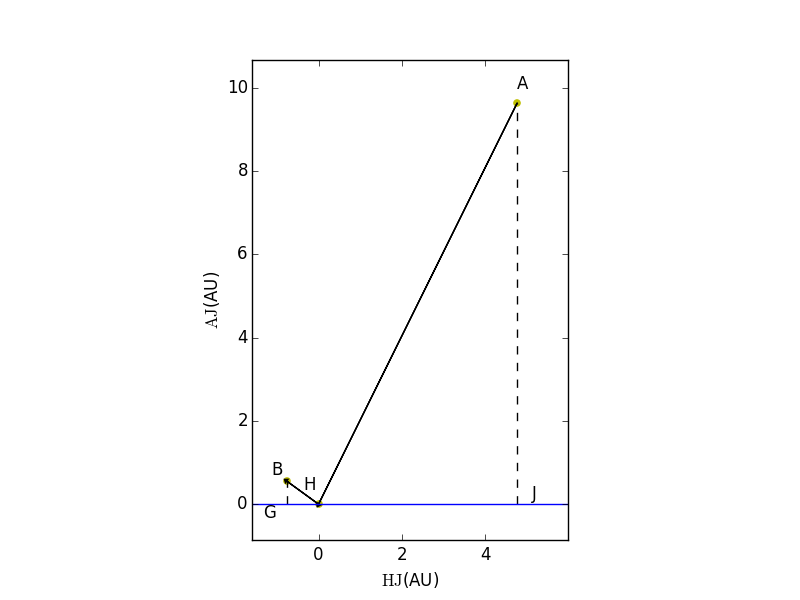
\includegraphics[width=1.0\linewidth,scale=1.0]{First_reflection.png}
\caption{Refraction on lens 2. 
%The x axis marks the distance in the direction that is parallel to lens 2, and the y axis marks the distance in the direction that is transverse to the lens 2. 
A is the position of the pulsar. H is the lensed image on lens 2. B is the lensed image on lens 1. J is the perpendicular of A to lens 2, and G is the perpendicular of B to lens 2. $v_{\rm JH}$ and $v_{\rm HG}$ should be equal, which is described in Section \ref{doublelensmodel}. In this case, $\theta_{1\parallel} =-17.39$ mas.}
\label{first_reflect}
\end{figure}

\begin{figure}
\centering
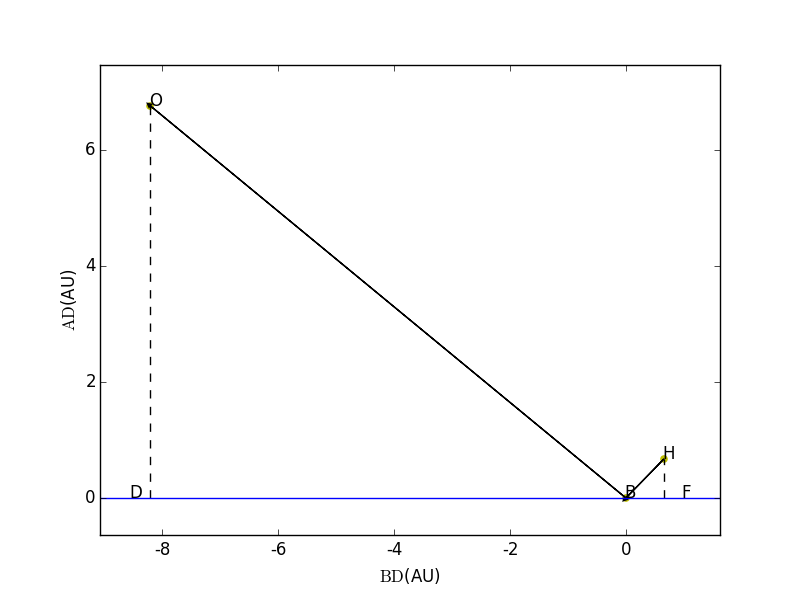
\includegraphics[width=1.0\linewidth]{Second_reflection.png}
\caption{Refraction on lens 1. 
%x axis marks the distance in the direction that is parallel to the second lens, and the y axis marks the distance in the direction that is transverse to the second lens. 
H is the lensed image on lens 2. B is the lensed image on lens 1. O is the position of the observer. F is the perpendicular of H to lens 2, and D is the perpendicular of O to lens 2. $v_{\rm FB}$ and $v_{\rm BD}$ should be equal, which is described in Section \ref{doublelensmodel}. In this case, $\theta_{1\parallel} = -17.39$ mas. }
\label{second_reflect}
\end{figure}



The solved positions are plotted in Figure \ref{Doublelens}, and respective time delays and differential frequencies are listed in Table \ref{table:double_lens_compare}. For the error of time delay $\tau$ in double lens model, we use the following equation: 
\begin{equation}
\begin{aligned}
(\frac{\sigma_{\tau_i}}{\tau_{2i}})^2 = (\frac{\sigma_{\tau1i}}{\tau_{1i}})^2+(\frac{\sigma_{\tau2i}}{\tau_{2i}})^2 + (\frac{\sigma_{\tau2j}}{\tau_{2j}})^2,
%\frac{\sigma_{\rm tot}}{\tau_2} = (\frac{\sigma_{\rm 1sample}}{\tau_1})^2+(\frac{\sigma_{\rm 2sample}}{\tau_2})^2,
\end{aligned}
\end{equation}
where $\tau_1$ and $\sigma_{\tau1}$ represent the time delay and its error from the $0.4$ ms group on lens $1$, $\tau_2$ and $\sigma_{\tau2}$ represent the time delay and its error from respective $1$ ms group on lens 2. And $\tau_{2j}$ is the $\tau_2$ for the nearest point in reference in Table \ref{table:double_lens_compare} and $\sigma_{\tau2j}$ is its error: for point $i=1,3$, $j=2$; for point $i=4$, $j=5$.
% $\tau_1$ is the time delay from $0.4$ ms group, and $\tau_2$ is the time delay from respective $1$ ms group.

For the error of differential frequency $f_D$, we use the following equation:
\begin{equation}
\begin{aligned}
(\frac{\sigma_{f_i}}{f_{Di}})^2=(\frac{\sigma_{f_{Di}}}{f_{Di}})^2+(\frac{\sigma_{f_{D2}}}{f_{D2}})^2
\end{aligned}
\end{equation}
where $f_{D2}$ and $\sigma_{f_{D2}}$ are the differential frequency and its error of the point in the second row in Table \ref{table:double_lens_compare}. $i=1,3,4,5$ for the subscription.

\subsubsection{Comparing model results in double lens model with observations}
Comparing $\tau$, we calculated time delay $\tau_M$ for these five points, and list the results in Table \ref{table:double_lens_compare}. For point 2 and 5, they fit perfectly because these are the two points that we use these to calculate the position of J; for the remaining three points, all of the calculated results are still within $3\sigma$ region of the observed time delays.

To compare differential frequency $f_D$, we need to calculate the
velocity of the pulsar and the velocity of the lens. We take the
lenses to be relative static, and solve for the velocity of the pulsar
relative to the lens.  The pulsar has two velocity components, and the
two 1-D lenses effectively determine one component each.
%To calculate the velocity of the pulsar, we need two components, the
%$v_{\parallel}$ in ${\parallel}$ direction, and $v_{\bot}$ in ${\bot}$
%direction.%, which is defined in Section \ref{subsec:angularpos}. 
For $v_{\parallel}$, we derive the velocity from $f_D$ of the $0.4$ ms
group in the one lens model, that is $179.8$ km/s.  The direct
observable is the time to crossing of each caustic, denoted $t_0$ in
Table \ref{table:apex}. 
%For the velocity of lens 2, because it is a line, and we do not consider radial velocity, so it could only be in the direction of AJ. However, $\angle$DAJ is $82\degree$ so $v_{\%bot}$ and $v_{\rm lens2}$ are nearly degenerate. In the following discussion, we consider lens 2 to be static and only take $v_{\bot}$ into account.

To calculate $v_{\bot}$, we choose the point 2, which has the smallest
errorbar of differential frequency.
% In a time period of $6500$ s, the
%$v_{\bot}$ is calculated to be $6.85$ km/s, in the direction pointing
%from B to D, to make the calculated $f_{D2}$ match the observation $f_D$. 
We find $v_{\rm tot}$ to be $192.4\pm 5.0$ km/s,
with an angle $\epsilon=4.34\degree$ west of north. The derived and
observed velocity are listed in Table \ref{Table:velocity}. The
direction of the model velocity is marked on the top of the star in
Figure \ref{Doublelens}.

\begin{table*}
\centering
\begin{tabular}{ccccc}
\hline
Parameter & $\mu_{\alpha*}$(mas/year) & $\mu_{\delta}$(mas/year) & $\mu_{l*}$(mas/year) & $\mu_b$ (mas/year)\\
\hline
model pulsar-screen velocity & $-4.84\pm 0.12$ & $63.4\pm 1.6$ & $-58.3$ & $23.2$ \\
%VLBI pulsar proper motion & $2.14 \pm 0.21$ & $51.64\pm 0.13$ & $45.32\pm 0.49$ %& $46.51 \pm 0.20$\\
VLBI pulsar proper motion & $2.14 \pm 0.21$ & $51.64\pm 0.13$ &
                                                                $-44.9$ & $25.6$\\
Screen motion &  &  & 13.4 & -2.4 \\
%pulsar proper motion (relative to earth) & $-7.52$ &  $53.5$ & $28.99$  & $52.1$ \\
%l=45.3157,44.8243,45.8071
%b=46.5138,46.3109,46.7166
\hline
\end{tabular}
\caption{Summary of velocities in double lens model. The screen is
  only moving slowly ($\sim 30$km/s).  Peculiar and earth motion were
  subtracted for galactic proper motion values.
}
\label{Table:velocity}
\end{table*}

%, which is also $\mu_\alpha=-4.84\pm0.12$ mas/year and $\mu_\delta=63.4\pm 1.6$ mas/year on equatorial plane. In galactic coordinate system the velocity is $\mu_l=41.87\pm 1.06$ mas/year, and $\mu_b=60.09 \pm 1.60$ mas/year. %note this part should be the (\mu_\alpha*cos(delta))^2+(\mu_delta)^2 should be the same.
%The error region of the velocity, which is determined by the error region of $f_D$ is $187.4-197.4$ km/s, the angular velocity region is $\mu_a=-4.71$-$-4.96$ mas/year and $\mu_d=61.8$-$65.1$ mas/year. 


With this velocity of the pulsar, we calculate the differential
frequency $f_M$ of point 1,3,4 and 5. Results are listed in Table
\ref{table:double_lens_compare}. The calculated results all lie in the
$3-\sigma$ region of the observation data. 



\begin{table*}
\centering
%\resizebox{\linewidth}{!}{
\begin{tabular}{llllllll}
\hline
$\theta_{1\parallel}$ (mas)  & $\tau_2$(ms) & $\sigma_{\rm \tau}$(ms)  & $\tau_M$(ms) & $f_D$(mHz)  &$\sigma_{f}$(mHz)      &  $f_M$(mHz)& $t_1$(days) \\ \hline
-13.82  &    0.9495     &0.0094    & 0.9550       & -35.1     &0.81    & -37.22          & -56\\ 
-14.59  &   0.9763    &0.00088   & 0.9763*       & -38.3     &0.64    & -38.31$\dagger$ & -60\\ 
-16.24  &   1.005    &0.011   & 1.027          & -40.17    &0.87   & -40.64          & -69\\ 
-16.52  &    1.0370     &0.0059    & 1.0363       & -41.27    &0.88   & -41.04          & -70\\ 
-17.39  &  1.0663     &0.0050    & 1.0663*        & -43.08    &0.84   & -42.27           & -75\\ \hline
\end{tabular}
%}
\caption{Comparison of time delay $\tau$ and the differential frequency $f_D$ of the observation and the calculated result in double lens model. $\theta_{1\parallel}$ denotes the angular offset of lens 1. 
%$\theta_{2\parallel}$ is the angle of the $1$ ms group with the component in the axis defined by $\gamma$. 
The values with star symbols on them are the points that we use to calculate the position of J and the point with a $\dagger$ symbol is the point that we use to calculate the velocity of the pulsar $v_{\rm A2}$. }
\label{table:double_lens_compare}
\end{table*}
%\end{table}



The reduced chi-square ${\chi}^2_{\nu}$ for time delay $\tau$ is $1.5$
for $3$ degrees of freedom
and $2.0$ for $f_D$ for $4$ degrees of freedom.  This is consistent
with the model.

%However, if the lines describing lens 1 are not parallel, there is
%still possibility that the differential frequency lie within the error
%region. For point 4 in double lens model, the angle between the axis
%of the $0.4$ ms group and the declination axis $\gamma$, should lie
%within the region 

Within this lensing model, we can test for the parallelness of the
caustics.  Using the lag error range of double lensed point 4 (the best
constrained), we find a $1-\sigma$ allowed angle of 0.4 degrees from
parallel with the whole lensing system.  This lends support of a
highly inclined sheet, probably aligned to better than 1\%.

%$\-25.2\degree \pm 0.4$ to meet the upper limit $f_{D4}+\sigma_{f4}$, $\tau_4+\sigma_{\tau 4}$ and the lower limit $f_{D4}-\sigma_{f4}$,$\tau_4-\sigma_{\tau 4}$ in Table \ref{table:double_lens_compare}, which has the smallest errorbar of the differential frequency.
%table one for 1ms positions

\subsubsection{Discussion of double lens model}
For $1$ ms group, lens 2
only images a subset of the lens 1 images.  This could happen if
lens 1 screen is just under the critical inclination
angle, such that only $3\sigma$ waves lead to a fold caustic.  If the lens 2 was at a critical angle, the chance of encountering a
somewhat less inclined system is of order unity.
%For the $0.4$ ms apexes, the one lens model could perfectly interpret the observation. 
More surprising is the absence of a single refraction
image of the pulsar, which is expected at position J.  This could
happen if the maximum refraction angle is just below critical, such
that only rays on the appropriately aligned double refraction can form
images.  
%This scenario predicts that at frequencies just below $300$
%MHz, or a few weeks earlier in time, the pulsar should be seen at
%position J. 
We plot the refraction angle $\beta$ in the
direction that is transverse to the first lens plane in Figure
\ref{vtrans}. The data
spans about 10\% in frequency, making it unlikely that single lens
image J would not be seen due to the larger required refraction
angle.  Instead, we speculate that the fold caustic could have formed
near double lens image 1, and thus only intersections with the closer
lens plane caustic south of image 1 are double lensed.

This is a generic outcome of a swallowtail
catastrophy\citep{Arnold1990}.   In this picture, the sheet just
starts folding near point 1.  North of point 1, no fold appears in
projection.  Far south of point 1, a full fold exhibits two caustics
emanating from the fold cusp.  Near the cusp the magnification is the
superposition of two caustics, leading to enhanced lensing and higher
likelihood of being observed.

We denote the time that the lensed image on lens 2 to move from point
H to point J, time $t_1$. From our calculation, $56$ days before the
lensed pulsar image to locate at J, it was at point 1; and $75$ days
before the lensed pulsar image to locate at J, it was at point 5. The
model predicts the presence of a single lensed image refracted at
these points, in addition to the double lenses images.

%test
%\begin{figure*}
%\centering
%\epsscale{1.0}
%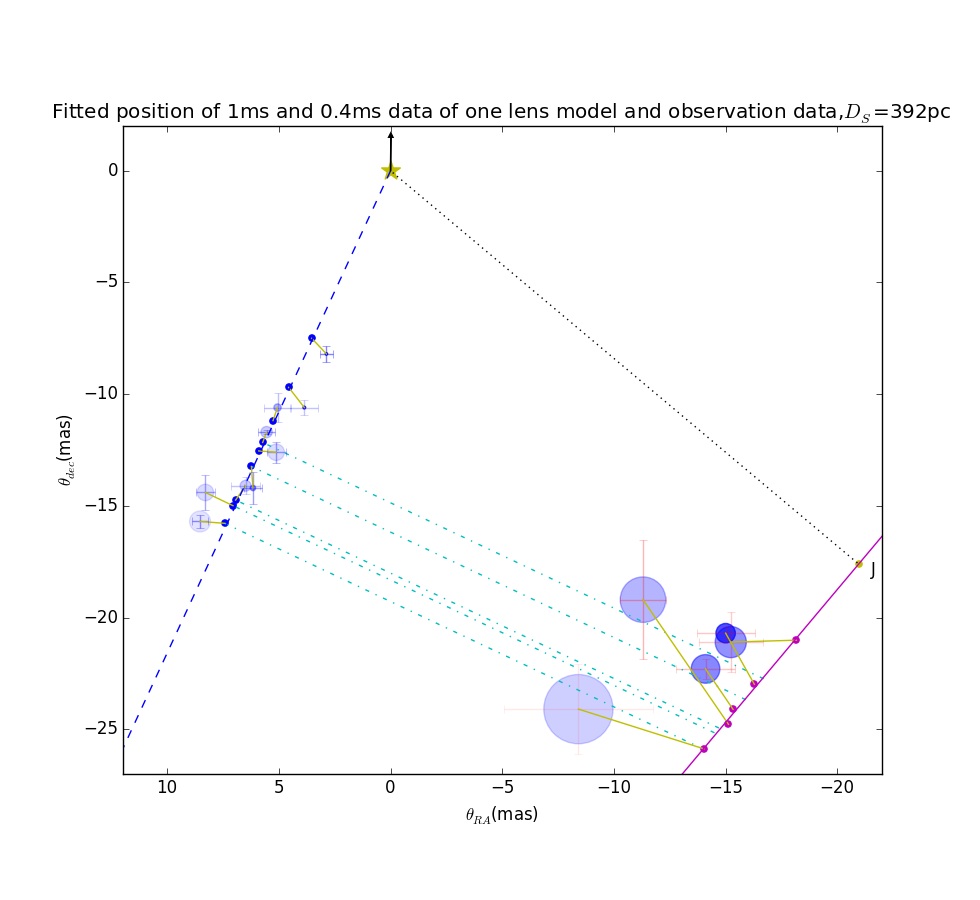
\includegraphics[width=0.8\textwidth, angle=0]{One_lens_640_392_392.png}
%\includegraphics{zN.eps}
%\caption{Fitted position of $1$ms and $0.4$ms data of one lens model and observation data. In both apexes regions, the position of the screen locate at $392.82$pc. Blue points on the left side are the points that fitted from the $f_D$ and $\tau$ of from the $0.4$ms observation. Blue line is the fitted line of $0.4$ms apex positions, with a $25.2$ degree west of the north. The points lie on the left side with errorbars, are the observation points together with their sample errors; while the transparent circles are plotted with population errors, where smaller transparent data are darker. Short solid lines between them are the matched positions of the apexes in $1ms$ region and $0.4ms$ region, which share the same $\theta_{\parallel}$. The points on the right side are the points that fitted from the $f_D$ and $\tau$ of the $1$ms observation with an avearage of four bandwidths. Solid line is the fitted line of these positions. Those points with errorbars nearby are the observation points together with their sample errors, while the transparent circles are plotted with population errors. The dotted line on the top right side is vertical to the solid line. Short solid lines connect the observation points and the fitted positions. Middle lines connect the $0.4$ms and $1$ms fitted positions with the same $\theta_{\parallel}$. The velocity of the pulsar is $199981$m/s, with a degree $0.0007$ radian east of north, which is marked out at the top of the figure.  }
%\label{Onelens_392}
%\end{figure*}

%\begin{figure*}
%\centering
%\epsscale{1.0}
%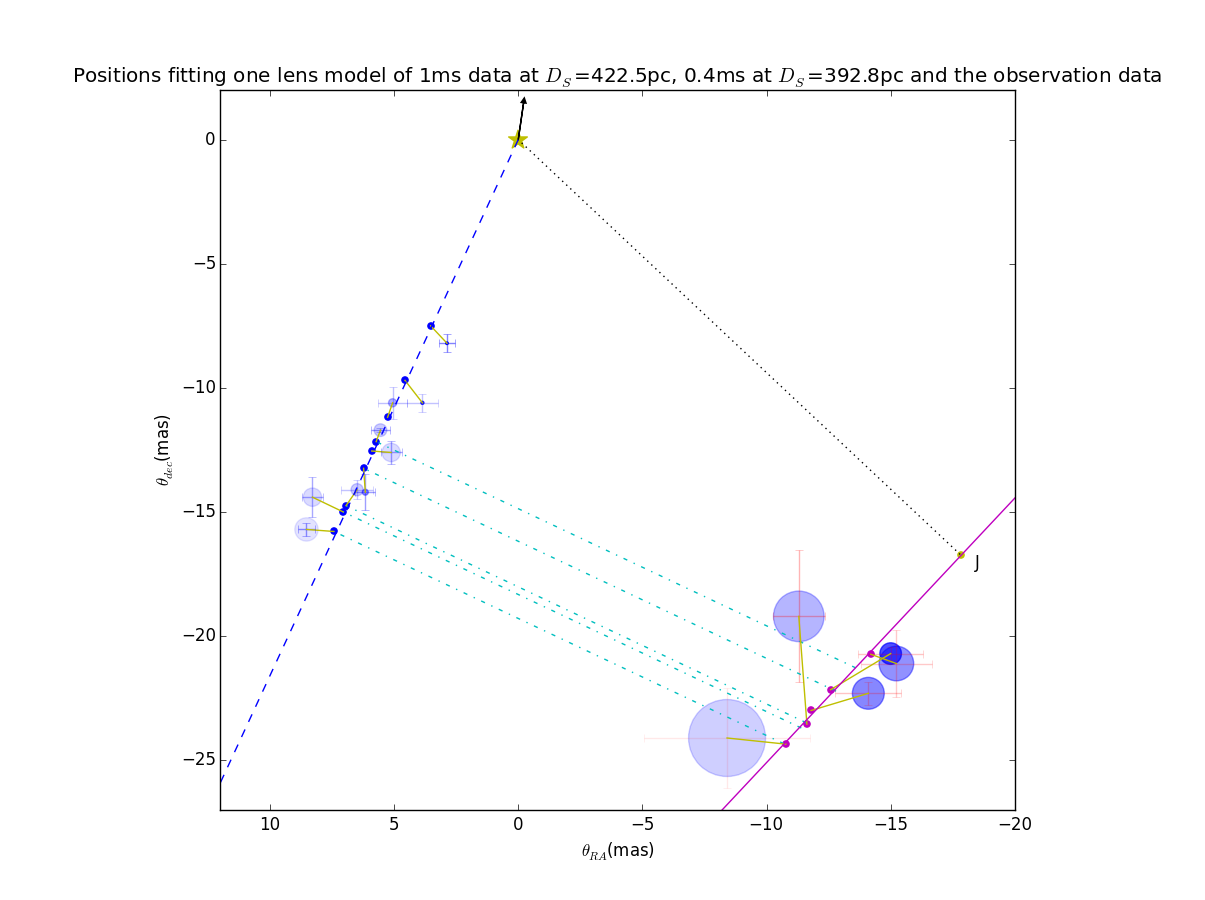
\includegraphics[width=0.8\textwidth, angle=0]{One_lens_640_392_422.png}
%\includegraphics{zN.eps}
%\caption{Same Observation data with the previous plot, this time we put the points with time delay lie in the range $1$ms at the screen that is $422.5$ pc away from us, which fitts better with the observation data. Velocity in this situation is $188499$m/s, with an angle $0.144147$ radian west of north. }
%\label{Onelens_392_422}
%\end{figure*}









%\begin{figure*}
%\centering
%\epsscale{1.0}
%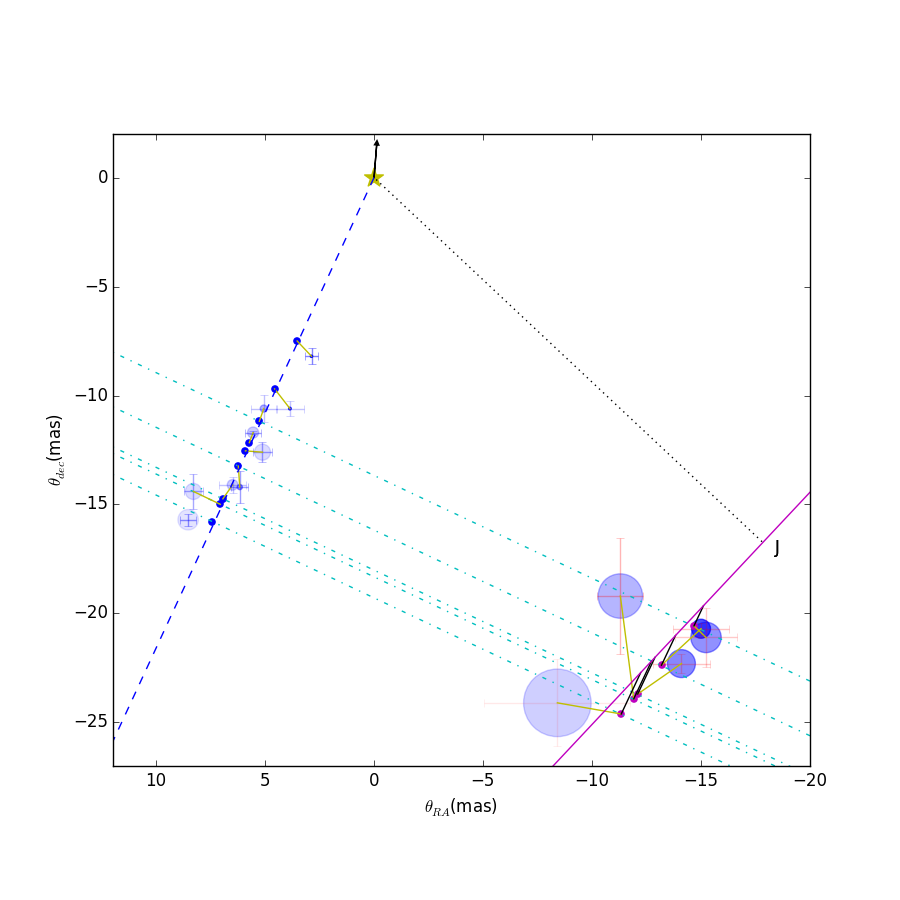
\includegraphics[width=1.0\textwidth, angle=0]{Double_lens_640_425_392.png}
%\caption{Fitted position of $1$ms and $0.4$ms data of double lens model and observation data.In both apexes regions, the position of the screen locate at $392.82$pc and $425$pc. Blue points on the left side are the points that fitted from the $f_D$ and $\tau$ of from the $0.4$ms observation. Blue line is the fitted line of $0.4$ms apex positions, with a $25.2$ degree west of the north. The points lie on the left side with errorbars, are the observation points together with their sample errors; while the transparent circles are plotted with population errors, where smaller transparent data are darker. Short solid lines between them are the matched positions of the apexes in $1ms$ region and $0.4ms$ region, which share the same $\theta_{\parallel}$. The points on the right side are the points that fitted from the $f_D$ and $\tau$ of the $1$ms observation with an avearage of four bandwidths. Solid line is the fitted line of these positions. Those points with errorbars nearby are the observation points together with their sample errors, while the transparent circles are plotted with population errors. The dotted line on the top right side is vertical to the solid line. Short solid lines connect the observation points and the fitted positions. Middle lines connect the $0.4$ms and $1$ms fitted positions with the same $\theta_{\parallel}$. The velocity of the pulsar is $191.4$km/s, with a degree $5.56$ degree west of north, is also marked out at the top of the figure.  }
%\label{Doublelens}
%\end{figure*}

\begin{figure}
\centering
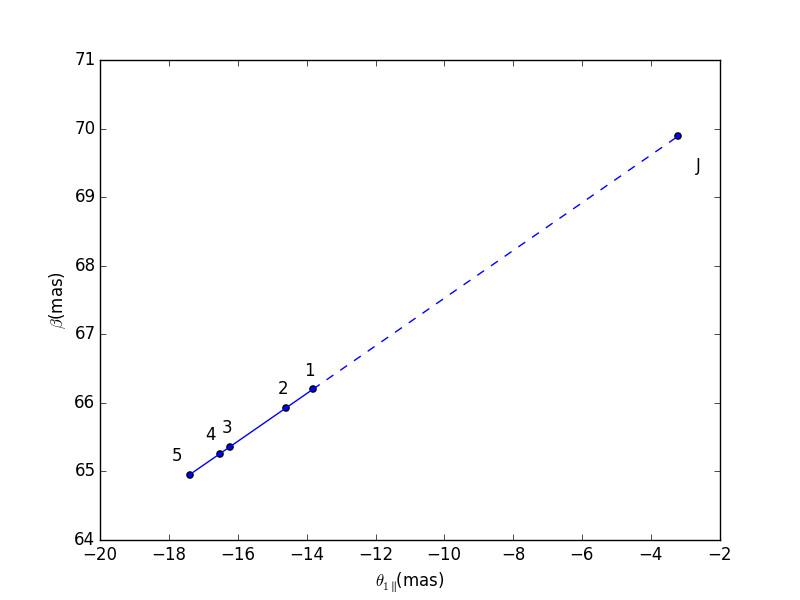
\includegraphics[width=1.0\linewidth]{Reflection_angle.png}
\caption{Deflection angle $\beta=\pi-\protect\angle$AHB on lens 2.  Point J denotes the expected
  deflected to form a single deflection image, which was not
  observed.   The small change in angle relative to the observed
  images precludes a finite refraction cutoff, since the data spans
  10\% bandwidth, with a 20\% change in refractive strength.  We
  propose a swallowtail caustic as the likely origin for the
  termination of the second lens sheet.
%  ($\pi$-$\protect\angle$AHB) vs $\theta_{1\parallel}$.
%vs $\theta_{\parallel}$.}
%$\beta_J$ is calculated with J as the lensed image on lens 2, when
%$\theta_{1\parallel}=-3.19$ mas.
}
\label{vtrans}
\end{figure}

\subsection{Distance Degeneracies}
\label{sec:degeneracy}
With two lens screens, the number of observables increases: in
principle one could observe both single reflection delays and angular
positions, as well as the double reflection delay and angular
position.  Three distances are unknown, equal to the number of
observables.  Unfortunately, these measurements are degenerate, which
can be seen as follows. From the two screens $i=1,2$, the two single
deflection effective distance observables are
$D_{i{\rm e}} \equiv c\tau_i/\theta_i^2=D_i^2(1/D_i+1/D_{pi})$.  A third
observable effective distance is that of screen 2 using screen 1 as a
lens, $D_{21{\rm e}}=D_1^2(1/D_1+1/D_{21})$, which is algebraically
derivable from the first two relations:
$D_{{21}{\rm e}}=D_{1{\rm e}}D_{2{\rm e}}/(D_{2{\rm e}}-D_{1{\rm e}})$.  

%This means that the distance
%to all subsequent lens screens can be inferred from time delays alone,
%and a measurement of the effective distances does not in fact add
%additional constraints.

In this archival data set the direct single lens from the further
plane at position J is missing.  It would have been visible $56$ days
earlier. The difference in time delays to image J and the double
reflection images would allow a direct determination of the effective
distance to lens plane 2.  Due to the close to 90 degree angle $\angle$DAJ
between lenses, the effect would be about a factor of 10 ill
conditioned.  with sufficiently precise VLBI imaging one could
distinguish if the double refracted images are at position B (if
screen 1 is closer) or position H.  As described above, we interpret
the effective distances to place screen 2 further away.

\section{Discussions}

\subsection{Interpretation}

The relative motion between pulsar and lens is directly measured by
the differential frequency, and not sensitive to details of this
model.  \citet{2010ApJ...708..232B}  derived similar motions.  This
motion is in broad agreement with direct VLBI proper motion
measurement, requiring the lens to be moving slowly compared to the
pulsar proper motion or the LSR.  The lens is $\sim$ 200 pc above the
galactic disk.  Matter can either be in pressure equilibrium, or in
free-fall, or some combination thereof.  In free fall, one expects
substantial motions.  These data rule out retrograde or radially
galactic orbits: the lens is corotating with the galaxy.  The modest
lens velocities appear consistent with the general motion of the ISM,
driven by galactic fountains\citep{1976ApJ...205..762S} at these
latitudes above the disk.
In the inclined sheet model, the waves move at alvenic speed, but due
to the high inclination, will move sub percent of this speed in
projection on the sky, and completely neglible compared to other
sources of motion.

Alternative models, for example evaporating
clouds\citep{1998ApJ...498L.125W} or strange
matter\citep{2013PhLB..727..357P}, do not make clear predictions.  One
would expect higher proper motions from these freely orbiting sources,
larger future scintillation samples may constrain these models.

In order to incline one sheet randomly to better than 1\% requires of
order $10^4$ randomly placed sheets, i.e. many per parsec.  This sheet
extends for $\sim$ 10 AU in projection, corresponding to a physical
scale greater than $1000$ AU.   These two numbers roughly agree,
leading to a physical picture of magnetic domain boundaries every
$\sim$ 0.1 pc.  B0834+06 has had noted arcs for multiple years,
perhaps suggesting this dominant lens plane is larger than typical.
One might expect to reach the end of the sheet within decades.

A generic prediction of the inclined sheets is a change in rotation
measure across the scattering length.  Over 1000 AU, one might expect
a typical RM change of $10^{-3}$ rad/m$^2$.  At low frequencies, for
example in LOFAR or GMRT, the size of the scattering screen extends
another order of magnitude in angular size, and RM changes increase to
$\sim 0.01$, which is plausibly measurable.

\subsection{Possible Improvements}

We discuss several strategies which can improve on the solution
accuracy.  The single biggest improvement would be to monitor over
several months, as the pulsar crosses each individual lens,
including both lensing systems.  This allows a direct comparison of
single lens to double lens arclets.

Angular resolution can be improved using longer baselines, for example
adding a GMRT-GBT baseline doubles the resolution.  Observing at
multiple frequencies over a longer period allows for a more precise
measurement: when the pulsar is between two lenses, the refraction
angle $\beta$ is small, and one expects to see the lensing at higher
frequency, where the resolution is higher, and distances between
lens positions can be measured to much higher accuracy.

Holographic techniques \citep{2008MNRAS.388.1214W,2014MNRAS.440L..36P}
may be able to measure delays, fringe rates, and VLBI positions
substantially more accurately.  Combining these techniques, the
interstellar lensing could conceivably achieve distance measurements
an order of magnitude better than the current published effective
distance errors.  This could bring most pulsar timing array targets
into the coherent timing regime, enabling arc minute localization of
gravitational wave sources, lifting any potential source confusion.

Ultimately, the precision of the lensing results would be limited by
the fidelity of the lensing model.  In the inclined sheet model, the
images move along fold caustics.  The straightness of these caustics
depends on the inclination angle, which in turn depends on the
amplitude of the surface waves.  

\section{Conclusions}

We have applied the \citep{2014MNRAS.442.3338P} inclined
sheet model to archival apex data of PSR B0834+06.  The data is well
fit by two linear lensing screens, with nearly plane-parallel
geometry.  The second screen provides a precision test with 10
observables and 3 free parameters.  The model fits the data to 
non-trivial percent accuracy on 7 points.
This natural consequence of very smooth
reconnection sheets is an unlikely outcome of ISM turbulence.
These results, if extrapolated to multi-epoch observations of binary
systems, might result in accurate distance determinations and
opportunities for removing scattering induced timing errors.


\section{Acknowledgements}

We thank NSERC for support.


\newcommand{\araa}{ARA\&A}   % Annual Review of Astronomy and Astrophys.
\newcommand{\afz}{Afz}       % Astrofizica
\newcommand{\aj}{AJ}         % Astronomical Journal
\newcommand{\azh}{AZh}       % Astronomicekij Zhurnal
\newcommand{\aaa}{A\&A}      % Astronomy and Astrophysics
\newcommand{\aas}{A\&AS}     % Astronomy and Astrophys. Supplement Series
\newcommand{\aar}{A\&AR}     % Astronomy and Astrophysics Review
\newcommand{\apj}{ApJ}       % Astrophysical Journal
\newcommand{\apjs}{ApJS}     % Astrophysical Journal Supplement Series
\newcommand{\apjl}{ApJ}      % Astrophysical Journal Letters
\newcommand{\apss}{Ap\&SS}   % Astrophysics and Space Science
\newcommand{\baas}{BAAS}     % Bulletin of the American Astron. Society
\newcommand{\jaa}{JA\&A}     % Journal of Astronomy and Astrophysics
\newcommand{\mnras}{MNRAS}   % Monthly Notices of the Roy. Astron. Society
\newcommand{\nat}{Nat}       % Nature
\newcommand{\pasj}{PASJ}     % Publ. of the Astron. Society of Japan
\newcommand{\pasp}{PASP}     % Publ. of the Astron. Society of the Pacific
\newcommand{\paspc}{PASPC}   % Publ. Astron. Soc. Pacific Conf. Proc.
\newcommand{\qjras}{QJRAS}   % Quart. Journal of the Royal Astron. Society
\newcommand{\sci}{Sci}       % Science
\newcommand{\solphys}{Solar Physics}       % 
\newcommand{\sova}{SvA}      % Soviet Astronomy
\newcommand{\aap}{A\&A}
\newcommand\jcap{{J. Cosmology Astropart. Phys.}}%
\newcommand{\prd}{Phys. Rev. D}


\bibliography{distance}
\bibliographystyle{mn2e}


\label{lastpage}

\end{document}
